\subsection{UC13 - Creazione prodotto}
\begin{figure}[H]
  \centering
  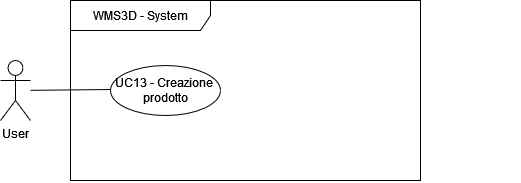
\includegraphics[width=0.8\textwidth]{UC_diagrams_11-20/UC13_sys.drawio.png}
   \caption{Diagramma UML UC13 - Creazione prodotto}
\end{figure}
\begin{figure}[H]
  \centering
  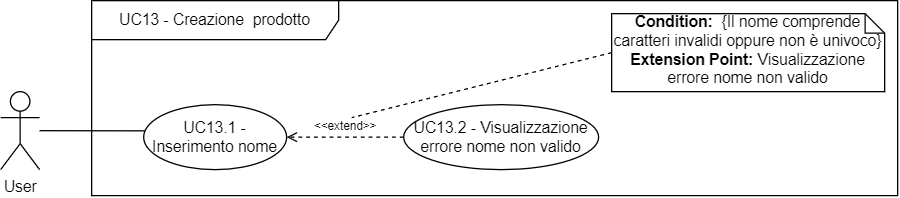
\includegraphics[width=0.8\textwidth]{UC_diagrams_11-20/UC13.drawio.png}
   \caption{Diagramma UML in dettaglio UC13 - Creazione prodotto}
\end{figure}
\begin{itemize}
    \item \textbf{Attori:} User.
    \item \textbf{Pre-condizione:}  L'utente ha creato/caricato un magazzino [UC1].
    \item \textbf{Post-condizione:} L'utente crea un prodotto che viene aggiunto in libreria\textsuperscript{G}.
    \item \textbf{Scenario Principale:}  L'utente crea un prodotto, inserendo un nome univoco [UC13.1] e delle dimensioni [UC13.2].
    \item \textbf{Generalizzazioni:} -
    \item \textbf{Estensioni:} -
\end{itemize}


\subsubsection{UC13.1 - Inserimento nome}
\begin{itemize}
    \item \textbf{Attori:} User.
    \item \textbf{Pre-condizione:}  L'utente ha creato/caricato un magazzino [UC1] e vuole creare un prodotto.
    \item \textbf{Post-condizione:} L'utente ha dato un nome identificativo al nuovo prodotto.
    \item \textbf{Scenario Principale:}  L'utente inserisce un nome univoco per il nuovo prodotto.
    \item \textbf{Generalizzazioni:} -
    \item \textbf{Estensioni:} È presente una estensione:
    \begin{itemize}
        \item UC13.3 - Visualizzazione errore nome non valido.
    \end{itemize}
\end{itemize}


\subsubsection{UC13.2 - Inserimento dimensioni}
\begin{figure}[H]
  \centering
  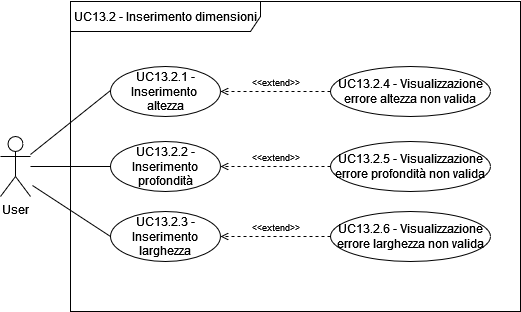
\includegraphics[width=0.8\textwidth]{UC_diagrams_11-20/UC13.2.drawio.png}
   \caption{Diagramma UML UC13.2 - Inserimento dimensioni}
\end{figure}
\begin{itemize}
    \item \textbf{Attori:} User.
    \item \textbf{Pre-condizione:}  L'utente ha creato/caricato un magazzino [UC1] e vuole creare un prodotto.
    \item \textbf{Post-condizione:} L'utente ha dato delle dimensioni al nuovo prodotto.
    \item \textbf{Scenario Principale:}  L'utente inserisce le dimensioni altezza [UC13.2.1], profondità [UC13.2.2] e larghezza [UC13.2.3] per il nuovo prodotto.
    \item \textbf{Generalizzazioni:} -
    \item \textbf{Estensioni:} -
\end{itemize}


\paragraph{UC13.2.1 - Inserimento altezza}
\begin{itemize}
    \item \textbf{Attori:} User.
    \item \textbf{Pre-condizione:}  L'utente ha creato/caricato un magazzino [UC1] e vuole creare un prodotto.
    \item \textbf{Post-condizione:} L'utente ha fornito l'altezza del nuovo prodotto.
    \item \textbf{Scenario Principale:}  L'utente inserisce l'altezza per il nuovo prodotto.
    \item \textbf{Generalizzazioni:} -
    \item \textbf{Estensioni:} È presente una estensione:
    \begin{itemize}
        \item UC13.2.4 - Visualizzazione errore altezza non valida.
    \end{itemize}
\end{itemize}


\paragraph{UC13.2.2 - Inserimento profondità}
\begin{itemize}
    \item \textbf{Attori:} User.
    \item \textbf{Pre-condizione:}  L'utente ha creato/caricato un magazzino [UC1] e vuole creare un prodotto.
    \item \textbf{Post-condizione:} L'utente ha fornito la profondità del nuovo prodotto.
    \item \textbf{Scenario Principale:}  L'utente inserisce la profondità per il nuovo prodotto.
    \item \textbf{Generalizzazioni:} -
    \item \textbf{Estensioni:} È presente una estensione:
    \begin{itemize}
        \item UC13.2.5 - Visualizzazione errore profondità non valida.
    \end{itemize}
\end{itemize}


\paragraph{UC13.2.3 - Inserimento larghezza}
\begin{itemize}
    \item \textbf{Attori:} User.
    \item \textbf{Pre-condizione:}  L'utente ha creato/caricato un magazzino [UC1] e vuole creare un prodotto.
    \item \textbf{Post-condizione:} L'utente ha fornito la larghezza del nuovo prodotto.
    \item \textbf{Scenario Principale:}  L'utente inserisce la larghezza per il nuovo prodotto.
    \item \textbf{Generalizzazioni:} -
    \item \textbf{Estensioni:} È presente una estensione:
    \begin{itemize}
        \item UC13.2.6 - Visualizzazione errore larghezza non valida.
    \end{itemize}
\end{itemize}


\paragraph{UC13.2.4 - Visualizzazione errore altezza non valida}
\begin{itemize}
    \item \textbf{Attori:} User.
    \item \textbf{Pre-condizione:}  L'altezza specificata del prodotto supera l'altezza del bin\textsuperscript{G} della scaffalatura.
    \item \textbf{Post-condizione:} L'utente visualizza un messaggio d'errore e l'operazione fallisce.
    \item \textbf{Scenario Principale:}  L'utente visualizza un messaggio informativo sull'errore e ne conferma la ricezione. L'operazione fallisce e l'utente dovrà scegliere una nuova altezza valida.
    \item \textbf{Generalizzazioni:} -
    \item \textbf{Estensioni:} -
\end{itemize}


\paragraph{UC13.2.5 - Visualizzazione errore profondità non valida}
\begin{itemize}
    \item \textbf{Attori:} User.
    \item \textbf{Pre-condizione:} La profondità specificata del prodotto supera la profondità del bin\textsuperscript{G} della scaffalatura.
    \item \textbf{Post-condizione:} L'utente visualizza un messaggio d'errore e l'operazione fallisce.
    \item \textbf{Scenario Principale:}  L'utente visualizza un messaggio informativo sull'errore e ne conferma la ricezione. L'operazione fallisce e l'utente dovrà scegliere una nuova profondità valida.
    \item \textbf{Generalizzazioni:} -
    \item \textbf{Estensioni:} -
\end{itemize}


\paragraph{UC13.2.5 - Visualizzazione errore larghezza non valida}
\begin{itemize}
    \item \textbf{Attori:} User.
    \item \textbf{Pre-condizione:}  La larghezza specificata del prodotto supera la larghezza del bin\textsuperscript{G} della scaffalatura.
    \item \textbf{Post-condizione:} L'utente visualizza un messaggio d'errore e l'operazione fallisce.
    \item \textbf{Scenario Principale:}  L'utente visualizza un messaggio informativo sull'errore e ne conferma la ricezione. L'operazione fallisce e l'utente dovrà scegliere una nuova larghezza valida.
    \item \textbf{Generalizzazioni:} -
    \item \textbf{Estensioni:} -
\end{itemize}


\subsubsection{UC13.3 - Visualizzazione errore nome non valido}
\begin{itemize}
    \item \textbf{Attori:} User.
    \item \textbf{Pre-condizione:}  L'utente ha inserito un nome identificativo di un prodotto che contiene caratteri invalidi oppure non è univoco.
    \item \textbf{Post-condizione:}  L'utente visualizza un messaggio d'errore e dovrà reinserire un nome diverso.
    \item \textbf{Scenario Principale:}  L'utente visualizza un messaggio informativo sull'errore e ne conferma la ricezione. L'operazione fallisce e l'utente dovrà scegliere un nuovo nome.
    \item \textbf{Generalizzazioni:} -
    \item \textbf{Estensioni:} -
\end{itemize}